\documentclass[11pt,a4paper]{article}


%KAP
% for including other TEX
\usepackage{standalone}
% for Unicode
\usepackage{ucs}
\usepackage[utf8x]{inputenc}
\usepackage{fontspec} % loaded by polyglossia, but included here for transparency
\usepackage{polyglossia}


%\usepackage{pdfpages}

% for tilde
\DeclareTextCommandDefault{\nobreakspace}{\leavevmode\nobreak\ } 

% for mathbb
\usepackage{amssymb}
% for "problem" environment
%\usepackage{amsthm}
\usepackage{thmtools}
% for {enumerate}[(1)]
\usepackage{enumerate}
% for noserif headings
%% \usepackage{sectsty} 
%\usepackage[sf,pagestyles]{titlesec} % make section headings \sffamily
% make headers \sffamily
%%\newpagestyle{main}[\sffamily]{
%%    \sethead{\thepage}{}{\sectiontitle}
%%    }
%%\pagestyle{main}
\usepackage{titling}
% make titling elements \sffamily
\pretitle{\begin{center}\sffamily\LARGE}
\preauthor{\begin{center}
            \large\sffamily \lineskip 0.5em%
            \begin{tabular}[t]{c}}
\predate{\begin{center}\sffamily\large}





\usepackage[margin=0.7in]{geometry}
\usepackage[usenames, dvipsnames]{color}
\usepackage{float}      % Required for proper figure placement
\usepackage{morefloats} % Required for proper figure placement
\usepackage{colortbl}
\usepackage{array}
\usepackage{multirow}
\usepackage{hyperref}
\usepackage{fancyvrb}   % For highlighted boxes in text
\usepackage{listings}   % Another way to quote verbatim
\usepackage{xcolor}
\usepackage{newverbs}   % Related to fancyvrb
\usepackage{amsmath}    % Required for arrows
\usepackage{mathtools}
\usepackage{textcomp}
\usepackage[section]{placeins} % Required for proper figure placement
\usepackage{graphicx}
\usepackage{adjustbox}  % Required to place graphics in lists
% \usepackage{sectsty}
\usepackage{titlesec}
\usepackage{lipsum}
\usepackage{etoolbox}
\makeatletter
\preto{\@verbatim}{\topsep=0pt \partopsep=0pt }
\makeatother




\usepackage{amsmath,amssymb}  
\usepackage{etoolbox}  
\usepackage[amsmath,framed,thmmarks]{ntheorem}  
\usepackage{thmtools}

\usepackage{pdfpages}
\usepackage{xcolor}


%KAP - is this chunk redundant?

%%%%%% New command to insert figures faster
\newcommand{\ra}{\begin{math}\rightarrow\,\end{math}}
\newcommand{\listfig}[2]{
    \begin{figure}[H]\centering
        \includegraphics[scale=0.6]{images/#1.png}
    \caption{#2}
    \label{fig:}
\end{figure}}
%%%%%% Use THIS command, rather than the previous.  Both work, but this one is cleaner
%%%%%% This takes two arguments, the name of the screenshot and the caption.  The screenshot must be png
%%%%%% Usage: \lfig{name-of-screenshot}{caption}
\newcommand{\lfig}[2]{
    \begin{figure}[H]\centering
        \includegraphics[scale=0.6]{images/#1.png}
    \caption{#2}
    \label{fig:}
\end{figure}}


% https://tex.stackexchange.com/questions/131726/conditional-content
% Display the argument if \cond is True/False
%\newcommand{\IfCond}[2]{%
%  \ifnum\pdfstrcmp{\cond}{True}=0
%    \ifnum\pdfstrcmp{}{#1}=0\unskip\else#1\fi%
%  \else
%    \ifnum\pdfstrcmp{}{#2}=0\unskip\else#2\fi%
%  \fi\ignorespaces}


\newcommand\invisiblesection[1]{%
  \refstepcounter{section}%
  \addcontentsline{toc}{section}{\protect\numberline{\thesection}#1}%
  \sectionmark{#1}}


%% KAP
\declaretheoremstyle[headfont=\normalfont\bfseries,notefont=\mdseries\bfseries,bodyfont = \normalfont,headpunct={:}]{normalhead}

\theorembodyfont{\normalfont}
\theoremheaderfont{\normalfont\bfseries}
\theoremseparator{.}
\theoremprework{\setlength
\theorempreskipamount{0 pt}\setlength\theorempostskipamount{0 pt}}


\newtheorem{innercustomthm}{Uzd.}
\newenvironment{problem}[1]
  {\renewcommand\theinnercustomthm{#1}\innercustomthm}
  {\endinnercustomthm}


\newcounter{alphnum}
\newenvironment{alphlist}{\begin{list}{(\Alph{alphnum})}{\usecounter{alphnum}\setlength{\leftmargin}{2.5em}} \rm}{\end{list}}

%% KAP: A4 papersizes:
\oddsidemargin 0.0in
\evensidemargin 0.0in
\textwidth 6.27in
\headheight 1.0in
\topmargin 0.0in
\headheight 0.0in
\headsep 0.0in
\textheight 9.69in
%\textheight 9.00in



%%%%%% To get highlighted boxes in text
\newverbcommand{\cverb}{\color{red}}{}
\newverbcommand{\grayverb}
  {\begin{lrbox}{\verbbox}}
  {\end{lrbox}\colorbox{gray!30}{\box\verbbox}}
\newverbcommand{\magverb}
  {\begin{lrbox}{\verbbox}}
  {\end{lrbox}\colorbox{magenta!30}{\box\verbbox}}
\newverbcommand{\yelverb}
  {\begin{lrbox}{\verbbox}}
  {\end{lrbox}\colorbox{yellow!30}{\box\verbbox}}
\newverbcommand{\blueverb}
  {\begin{lrbox}{\verbbox}}
  {\end{lrbox}\colorbox{blue!30}{\box\verbbox}}

%%%%%% Define Forcepoint Green
\definecolor{FP-Green}{RGB}{56, 163, 32}
% \sectionfont{\fontsize{18}}

%%%%%% Define colors for sections
\titleformat*{\section}{\Large\sffamily\bfseries\color{FP-Green}}
\titleformat*{\subsection}{\large\sffamily\bfseries\color{FP-Green}}
\titleformat*{\subsubsection}{\large\sffamily\bfseries\color{FP-Green}}

%%%%%% Place Draft as a watermark for review
% \usepackage{draftwatermark}
% \SetWatermarkText{INTERNAL ONLY}          %uncomment for watermarks
% \SetWatermarkColor[gray]{0.9}
% \SetWatermarkScale{2}
% \SetWatermarkAngle{0}
% \usepackage{mathtools}
% \usepackage{amsmath}

%%%%%% Example of figures in lists
%    \begin{minipage}[t]{\linewidth}
%                    \raggedright
%                    \adjustbox{valign=t}{%
%                    %\includegraphics[width=.8\linewidth]{ScreenShots/Policy-button.png}%
%                    \includegraphics[scale=0.6]{ScreenShots/Policy-button.png}%
%                    }
%                    \medskip
%            \end{minipage}
% Using figures
% \begin{figure}[ht]\centering
%      \includegraphics[scale=0.4]{ScreenShots/Key-field-mapping.png}
% \end{figure}

\setcounter{section}{0}


\title{\Huge\bfseries \color{FP-Green}Baltic Way, Skaitļu teorija}
\author{Neklātienes matemātikas skola}
\date{\today}
\begin{document}
%\maketitle % make title page.  Comment out if not desired

\begin{center}
{\LARGE Walk-Through:  Testing Machine on VirtualBox}
\end{center}


\begin{abstract}
Jenkins is a continuous integration tool with many extensions that 
allows to standardize the project lifecycle: it ensures that appropriate
revision of the project is used for the current build, that the software is tested 
accordingly to expected schedule and the testing results are summarized in a
user-friendly report. We will use this setup to grade your C++ exercises.

Using Jenkins by students is NOT mandatory. 
Jenkins is just the place where different tools such as GitHub, shellscripts, Makefiles, 
crontab scheduling, Web-based reporting can be put together. 
There are many other reasonable ways how you can integrate these tools \textendash{} you 
are encouraged to use whatever works for you. 
\end{abstract}

\section{Objectives}

Building and testing of student projects should be consistent to align 
expectations of students and instructors. 
The following features make Jenkins continuous build software a
good match for our C++ class.

\begin{description}
\item[Virtual Environment] \hfill \\
Run C++ projects in an environment with standardized 
operating system and its environment variables. VirtualBox and 
Xubuntu ensure this standardization. 
\item[Directory Layout] \hfill \\
Project files should have predictable layout; version control (such as GitHub) should 
be used to mark the submission, if possible.
\item[Execution Time] \hfill \\
Jenkins build steps can have timeout limitations so that C++ program execution is stopped, 
if it goes into an infinite loop or runs an inefficient algorithm.
\item[Scheduling Build Tasks] \hfill \\
Build steps (and also grading of student submissions) can be scheduled using crontab-like notation.
\item[User-Friendly Reporting] \hfill \\
If build tasks fail or tests do not match the expected files, this should be easy to see. 
\end{description}





\section{Walk-Through Outline}

This walk-through will consist of the following major steps (their detailed descriptions
follow in the next subsection).

\begin{enumerate}
\item Install VirtualBox software. Create a guest machine slot named {\tt Xubuntu} on VirtualBox. 
\item Create and configure Xubuntu guest machine.
\item Install basic software on the Xubuntu guest.
\item Set up Jenkins software on Xubuntu. 
\item Configure an additional Network Interface Controller (NIC) on guest machine 
to allow remote connection. 
\item Configure a build task on Jenkins and run it. 
\end{enumerate}






\section{Walk-Through Steps}

\subsection{VirtualBox Setup}

\begin{enumerate}
\item Visit \url{https://www.virtualbox.org/} and download the most recent 
VirtualBox installer. 
\begin{enumerate}[(a)]
\item Click on {\bf Download VirtualBox 6.1} banner. 
\item Click the link {\bf Windows hosts}, if your physical machine is Windows 10 laptop 
(or choose other operating system \textendash{} to whatever you have). 
\item Save the instler, such as {\bf VirtualBox-6.1.12-139181-Win.exe}. 
\end{enumerate}
\item Double-click on the VirtualBox installer (elevate privileges
to Admin-level, if asked to do so), and pick the default values to install it.
\item Run the newlly installed application {\bf Oracle VM VirtualBox}.\\
\frame{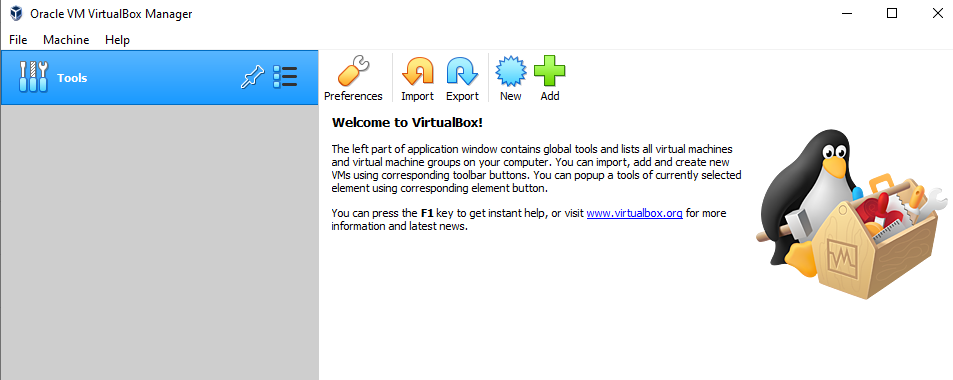
\includegraphics[width=5in]{virtualbox-walk-through/virtualbox1.png}}
\item Click button {\bf New} and enter the name of your new virtual guest, for example, {\tt xubuntu}.\\
\frame{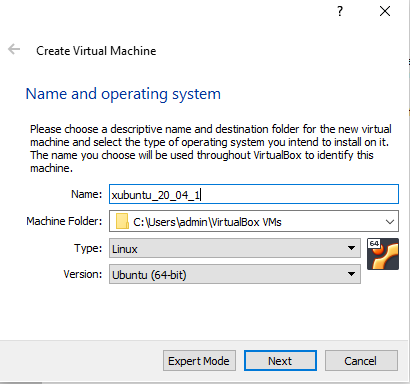
\includegraphics[width=3in]{virtualbox-walk-through/virtualbox2.png}}
\item Leave the default RAM memory size (1024 MiB). If your laptop is powerful (16 or more GiB of RAM), 
consider giving more RAM memory, say, 2048 MiB.
\item Leave the default option {\bf Create a virtual hard disk now}; also leave the {\bf VDI (VirtualBox Disk Image)}. 
\item Leave the default option {\bf Dynamically allocated}. 
\item Confirm the location of virtual memory image.\\[6pt]
\frame{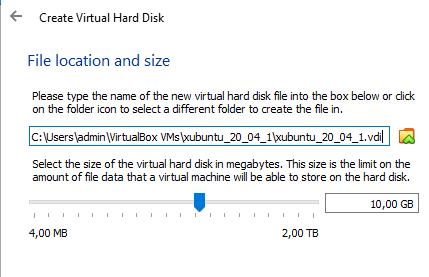
\includegraphics[width=3in]{virtualbox-walk-through/virtualbox7.png}}
\end{enumerate}



\subsection{Creating Xubuntu Guest}

\begin{enumerate}
\item Download the Xubuntu installer (as an ISO file of some stable release). 
Visit \url{https://xubuntu.org/download/} and pick a 64-bit ISO image.
In our example it is {\bf xubuntu-20.04.1-desktop-amd64.iso}. 
\item Make sure that the guest machine is powered off, 
select {\tt xubuntu} machine and click button {\bf Settings}. 
\item Under {\bf Settings} select {\bf Storage} $>$ {\bf Controller IDE} $>$ {\bf Empty}.\\
\frame{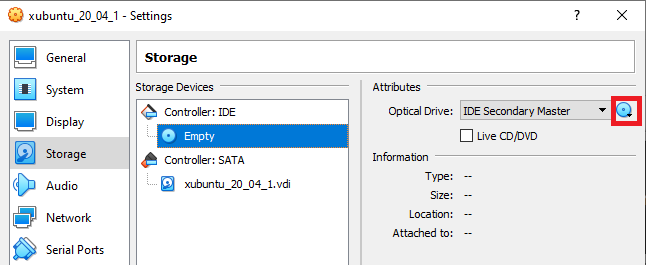
\includegraphics[width=3in]{virtualbox-walk-through/virtualbox9.png}}
\item Click on the browse button (highlighted in red in the above image). Select the
Xubuntu image that you downloaded earlier.\\
\item In the VirtualBox application, select the {\tt xubuntu} machine
and click on the button {\bf Run} (the green arrow).
\item Wait about 5 minutes until Xubuntu image loads from the virtual CD-ROM drive.
Click on the button {\bf Install Xubuntu}.\\
\frame{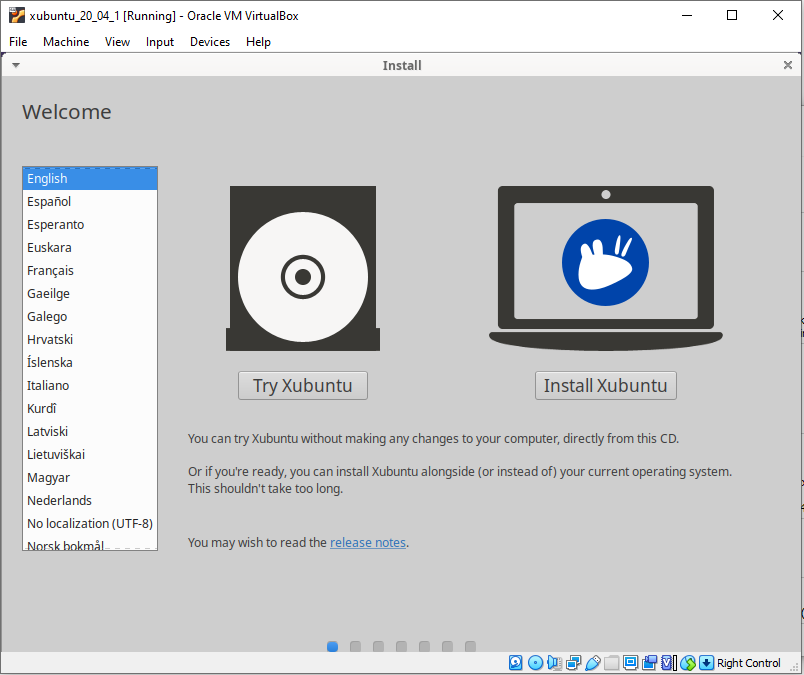
\includegraphics[width=3in]{virtualbox-walk-through/xubuntu3.png}}
\item Leave the default keyboard layout {\bf English (US)} $>$ {\bf English (US)}.
\item Selecting the checkbox {\bf Select third party software...} in the Xubuntu installer
is optional (it is selected on instructor machines).
\item Leave the default radio button {\bf Erase disk and install Xubuntu}.
\item Select {\bf Riga} as your current location.
\item Enter an Xubuntu Linux machine name (some short name with lower-case English letters such as 
{\tt miuse}), your username (e.g.\ {\tt 
student}) and some password (e.g. {\tt Bitl1!}).\\
\frame{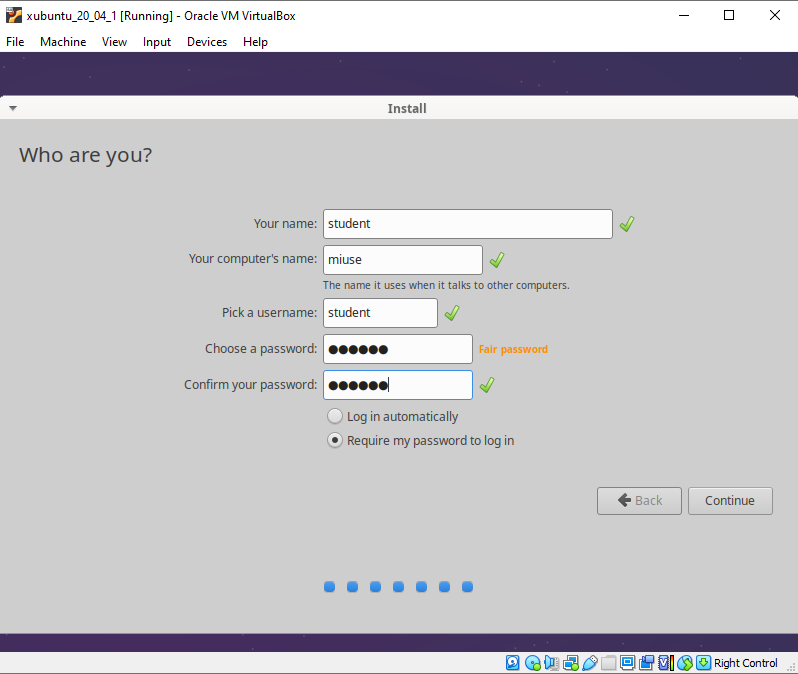
\includegraphics[width=3in]{virtualbox-walk-through/xubuntu7.png}}\\
\textcolor{red}{{\bf Note.} At this point you would need to wait about 15 minutes until VirtualBox finishes installing Xubuntu guest.} 
\item Reboot the machine. Log in as user {\tt student} and enter the password.
\item Click on the upper-left corner (the mouse-like Xubuntu start button) and start 
typing word {\tt terminal}. Once you see {\bf Terminal Emulator}, right-click it and 
select {\bf Add to Desktop}. This would make easier to create Linux-like terminal windows
and run command-lines.\\
\frame{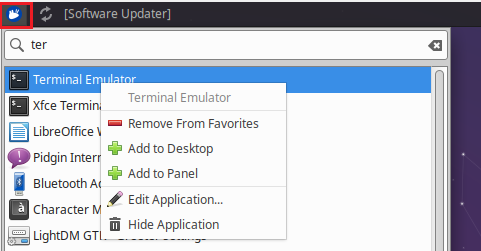
\includegraphics[width=3in]{virtualbox-walk-through/xubuntu9.png}}
\end{enumerate}


\subsection{Install Basic Software on Xubuntu}

\begin{enumerate}
\item Set the root password to {\tt Bitl1!} \textendash{} same as for the user {\tt student}:
\begin{verbatim}
sudo passwd   (enter Bitl1! password as student user)
    (type Bitl1! twice to set root's password)
\end{verbatim}
\item Install all the software updates:
\begin{verbatim}
sudo apt-get update
sudo apt-get upgrade
\end{verbatim}
\item Install Java JDK (prerequisite for Jenkins). First search all the ``openjdk'' related installations, 
then install the package {\tt openjdk-8-jdk}. Finally, check if your Java has the right version 1.8.
\begin{verbatim}
sudo apt search openjdk
sudo apt install openjdk-8-jdk
java -version
\end{verbatim}
\item Install C++ compiler (named {\tt g++}) and also {\tt make} utility:
\begin{verbatim}
sudo apt install build-essential
\end{verbatim}
\item Install Git client:
\begin{verbatim}
sudo apt-get install git
\end{verbatim}
\end{enumerate}



\subsection{Setup of Jenkins}

\begin{enumerate}
\item In the Xubuntu guest machine, click on the mouse-start button. Type in {\tt Web Browser}
to open Firefox-like browser. 
\item Find the Jenkins installation commands for Debian/Ubuntu. Type this URL into the browser:
\url{https://www.jenkins.io/doc/book/installing/#debianubuntu}.\\
Or, perhaps, Google search for {\tt install jenkins on ubuntu}:\\
\frame{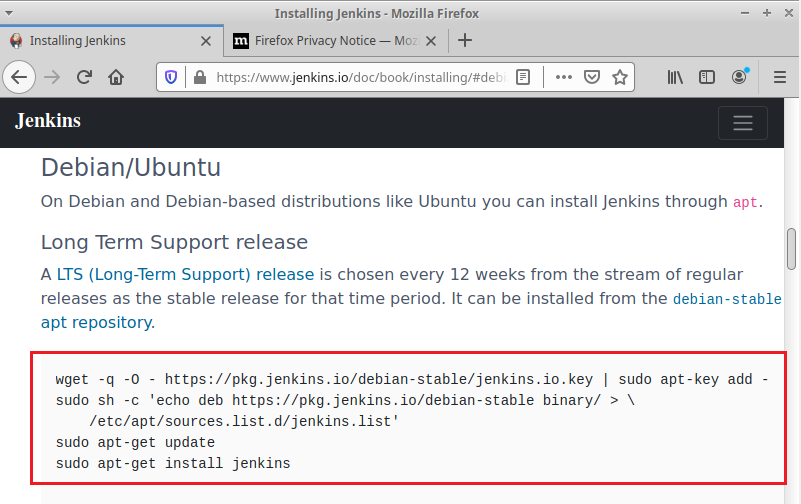
\includegraphics[width=3in]{virtualbox-walk-through/jenkins02.png}}
\item Copy-paste all the 4 commands into Xubuntu terminal (highlighted in red
rectangle in the above image).\\
\frame{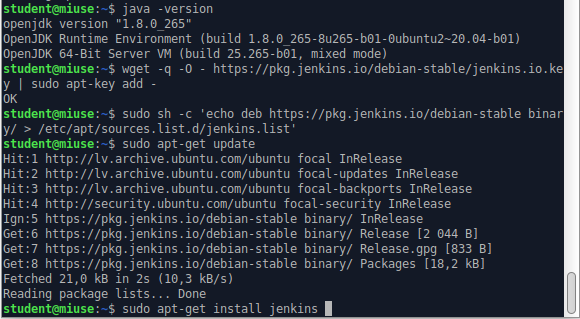
\includegraphics[width=3in]{virtualbox-walk-through/jenkins03.png}}
\item Register Jenkins as a system service that starts whenever Xubuntu is running:
\begin{verbatim}
sudo systemctlstart jenkins
sudo systemctl status jenkins
\end{verbatim}
\item In Xubuntu Web Browser enter {\tt http://127.0.0.1:8080}.\\
\frame{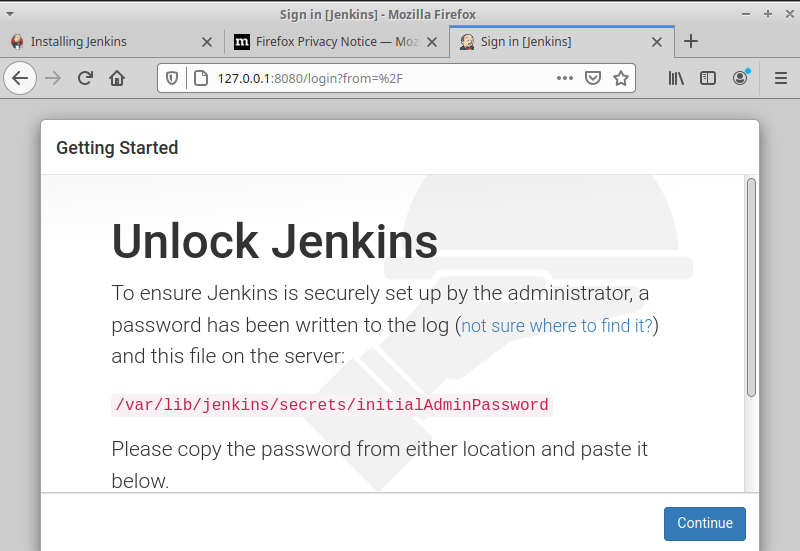
\includegraphics[width=3in]{virtualbox-walk-through/jenkins04.png}}
\item Change the user to {\tt root} using ``su - root'' command and display 
the file containing the initial password of Jenkins.\\
\frame{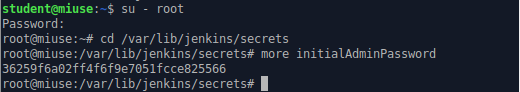
\includegraphics[width=2.5in]{virtualbox-walk-through/jenkins05.png}}
\item Copy-paste this one-time password into your browser, click {\bf Continue}.
\item If Jenkins offers to install all the usual plugins, close the screen.\\ 
\frame{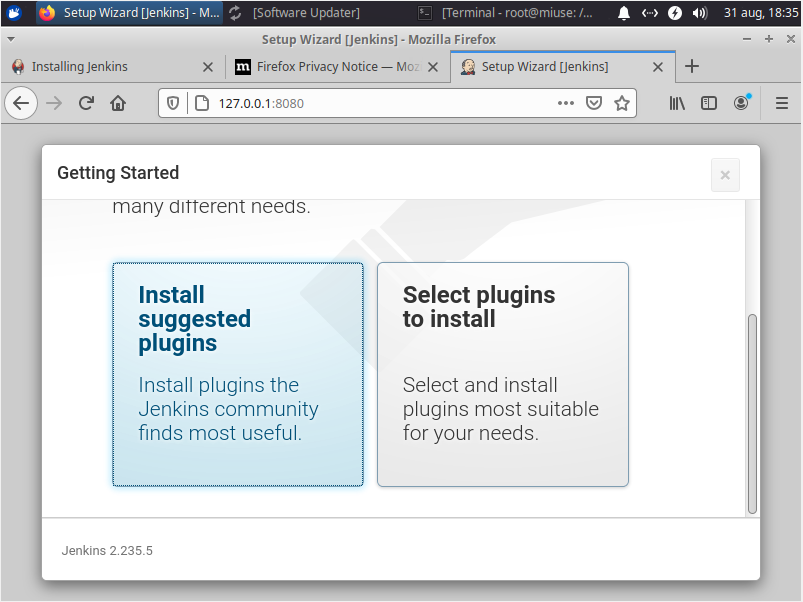
\includegraphics[width=3in]{virtualbox-walk-through/jenkins07.png}}\\
\textcolor{red}{{\bf Note.} Continuing with installing all the plugins 
might crash Jenkins instance.} 
\item Reopen Browser, log into Jenkins again. 
In the Jenkins Web interface open {\bf Manage Jenkins} $>$ {\bf Security} $>$ 
{\bf Manage Users} $>$ {\bf admin}.\\
\frame{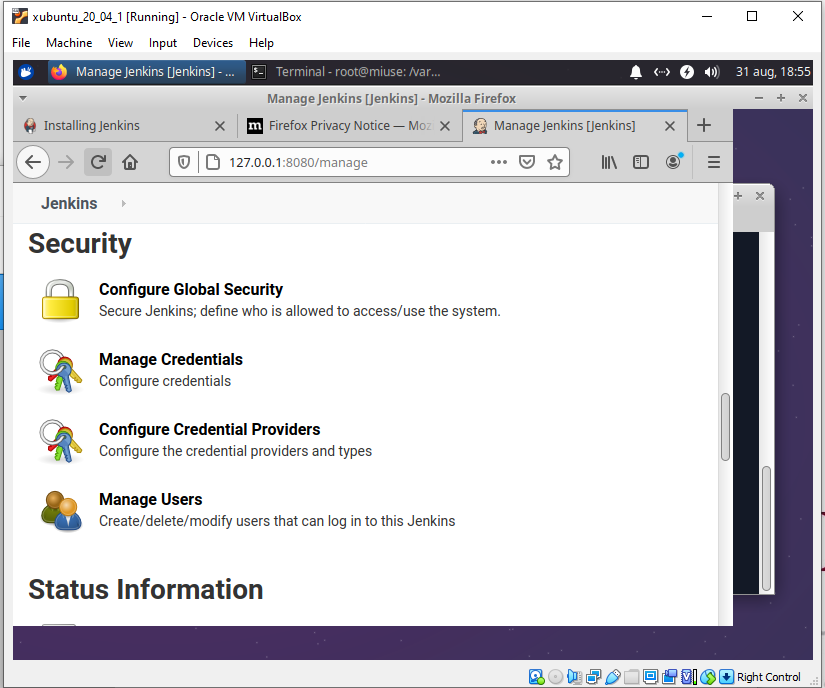
\includegraphics[width=3in]{virtualbox-walk-through/jenkins10.png}}
\item Change the password to something easier, say {\tt Bitl1!}\\
\frame{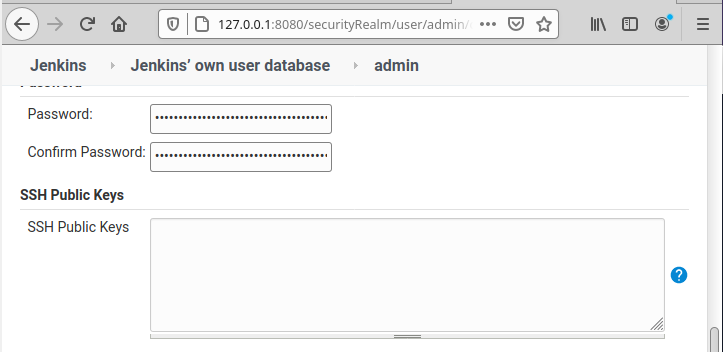
\includegraphics[width=3in]{virtualbox-walk-through/jenkins12.png}}
\item Navigate to {\bf Manage Jenkins} $>$ {\bf Manage Plugins}. 
Open tab {\bf Available}, search for the plugin {\bf GitHub} and install it.\\
\frame{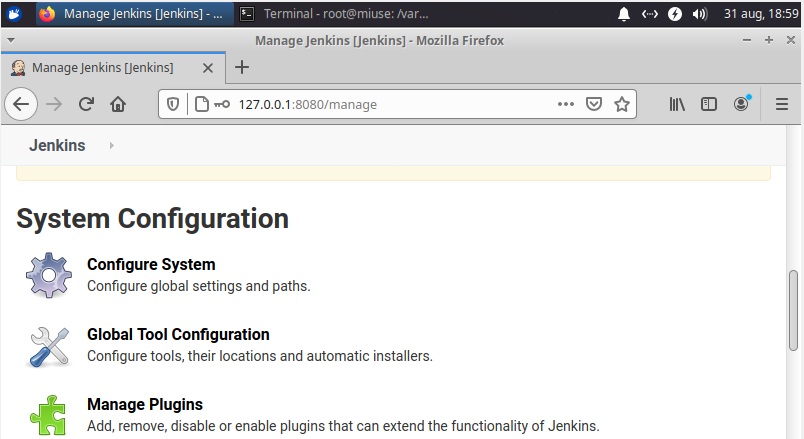
\includegraphics[width=3in]{virtualbox-walk-through/jenkins13.png}}
\end{enumerate}



\subsection{Fixing Host-Guest Networking}


\begin{enumerate}
\item Shut down the Xubuntu guest. 
\item In VirtualBox application open {\bf File} $>$ {\bf Host Network Manager} and 
inspect the host network router.\\
\frame{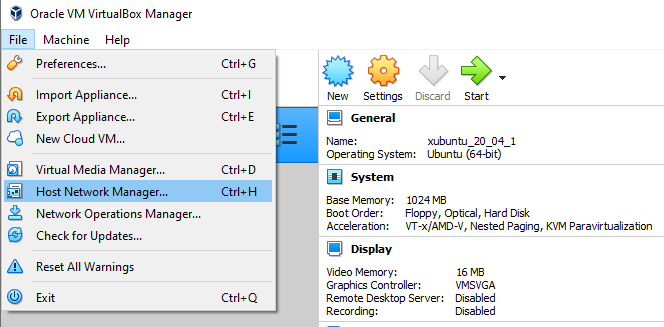
\includegraphics[width=3in]{virtualbox-walk-through/networking1.png}}
\item Select the (stopped) Xubuntu guest machine in VirtualBox and select {\bf Settings}.\\
\frame{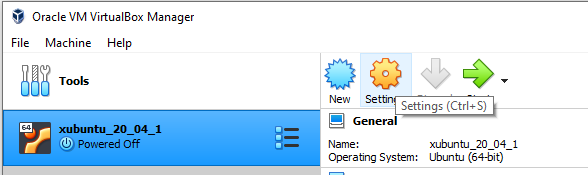
\includegraphics[width=3in]{virtualbox-walk-through/networking2.png}}
\item Open {\bf Network} $>$ {\bf Adapter 2}. Select the {\bf Enable Network Adapter} checkbox
and select {\bf Host-only Adapter} from the drop-down list.\\
\frame{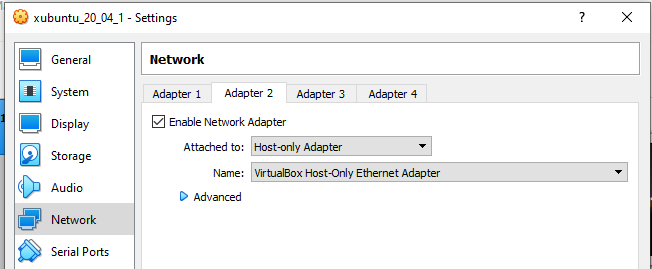
\includegraphics[width=3in]{virtualbox-walk-through/networking3.png}}
\item Run the Xubuntu guest machine (click on the green arrow).
\item Open terminal window on Xubuntu and run command {\tt ifconfig -a}\\
\frame{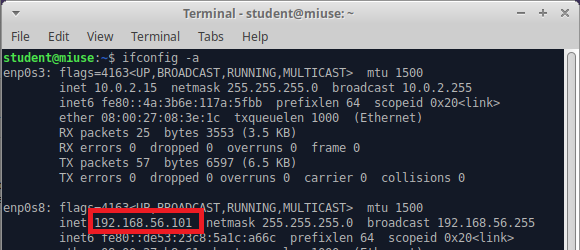
\includegraphics[width=3in]{virtualbox-walk-through/networking4.png}}
\item If you wish, open console on your host machine (such as Windows 10 or whatever). Type command
{\tt ipconfig /all}. You should be able to see a new network related to your VirtualBox.\\
\frame{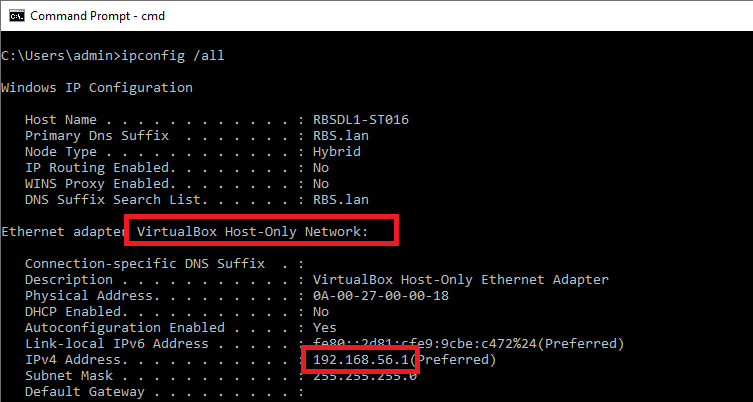
\includegraphics[width=3in]{virtualbox-walk-through/networking5.png}}
\item Use the Xubuntu address in the ``Host-only network'' to connect from your host machine. 
Open Chrome browser and type in address \url{http://192.168.56.101:8080}. \\
\frame{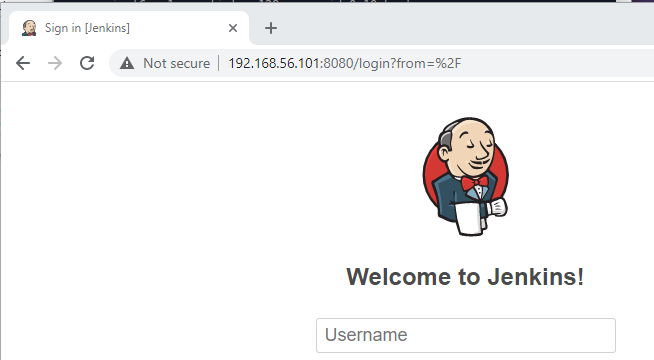
\includegraphics[width=3in]{virtualbox-walk-through/networking6.png}}
\item If Jenkins offers to make this URL to be ``the Jenkins URL'', agree by 
clicking {\bf Save and Finish}. Log in using the credentials {\tt admin} 
and {\tt Bitl1!}.
\end{enumerate}

\subsection{Configure and Run a Jenkins Task}


\begin{enumerate}
\item Create a private GitHub repository ({\tt workspace-cpp} in our example, but you can 
name it however you want). Create a subdirectory {\tt palindromes} containing 
some C++ sources and a makefile. You can copy the source code from this URL:\\
\url{http://linen-tracer-682.appspot.com/data-structures-bin/palindromes.zip}.
\item Share the repository URL with your instructor (and add him as 
\item Open \url{http://192.168.56.101:8080} and log in.
\item Enter some project name {\tt test01-palindromes}, select {\bf Freestyle project}.
\item Open tab {\bf Source Code Management}, enter the repository URL of your GitHub repository.\\
\frame{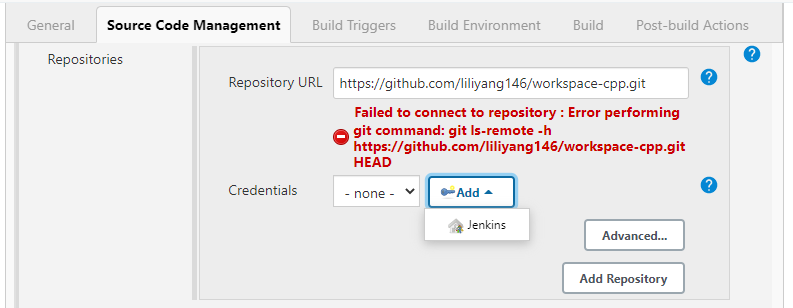
\includegraphics[width=3in]{virtualbox-walk-through/task4.png}}
\item A red warning should be displayed. Add the credentials to log into your private repository. 
(To keep your repository safe, do not share your Xubuntu/Jenkins instance with others.)\\
\frame{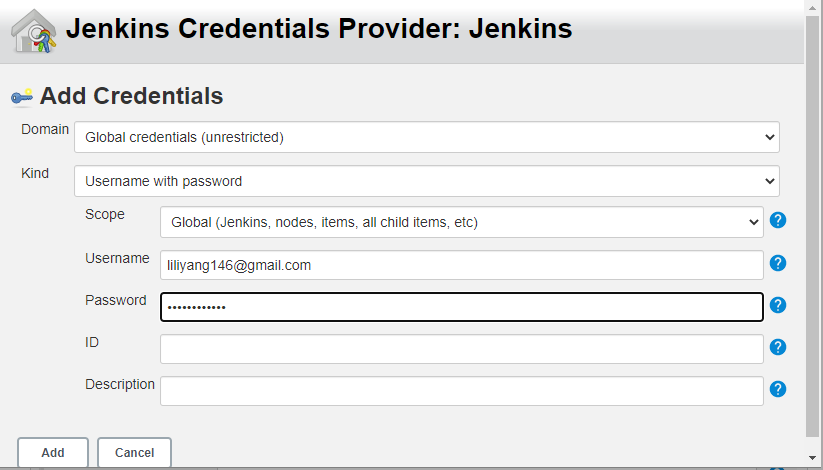
\includegraphics[width=3in]{virtualbox-walk-through/task5.png}}
\item Under subsection {\bf Build} create a new build script to execute once the code is
checked out from the GitHub repository.\\
\frame{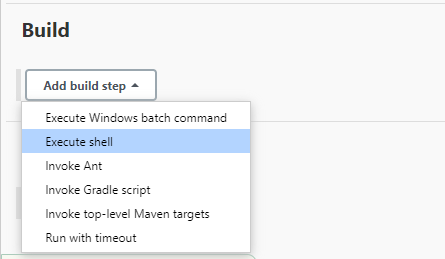
\includegraphics[width=3in]{virtualbox-walk-through/task7.png}}
\item Enter the following commands in the script editor:\\
\frame{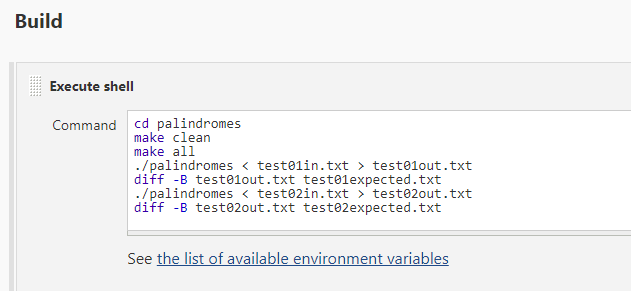
\includegraphics[width=3in]{virtualbox-walk-through/task8.png}}
\item Click on button {\bf Build Now} to execute your task.
\item You can inspect the {\bf Console Output} if it failed.\\
\frame{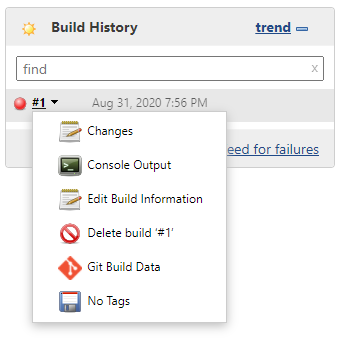
\includegraphics[width=3in]{virtualbox-walk-through/task10.png}}
\item The console commands with some output will be displayed on the browser screen:\\
\frame{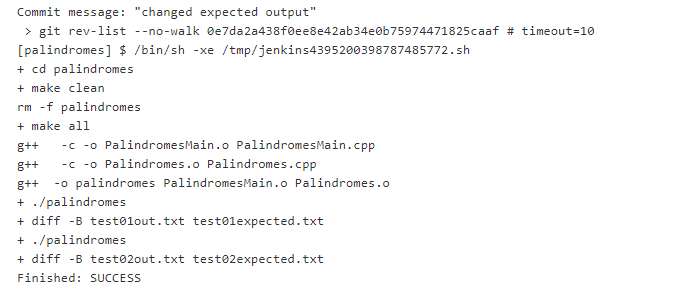
\includegraphics[width=3in]{virtualbox-walk-through/task12.png}}
\item If the console output is not sufficiently clear, you can locate the project in Jenkins 
workspace and run the build commands manually to find what is wrong.\\
\frame{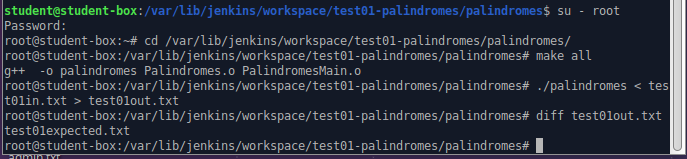
\includegraphics[width=4in]{virtualbox-walk-through/task13.png}}
\end{enumerate}



%(Running demo examples using one or more virtual guest images is a well-known 
%approach in IT education. A classical book (\cite{Stevens1994}, Section 1.16)
%introduced a preconfigured set of different machines to demonstrate various network protocols.)
%
%\begin{thebibliography}{9}
%\bibitem[Stevens1994]{Stevens1994} ``TCP/IP Illustrated'' by  W. Richard Stevens. Addison-Wesley, 1994. W. Richard Stevens.
%\url{https://bit.ly/3hM4WW0}.
%\bibitem[label2]{cite_key2} Cits kaut kas.
%\end{thebibliography}

\end{document}
